%%Template file, originally intended for an injection simulator school project at ETH Zurich. The file is based on IEEE transactions style
%Heike Vallery, January 2010, Zurich. Last update April 2021, Delft.
%Remark: Some packages may be outdated.
%Dez2022: Inhalt ins Deutsche übertragen und Anpassungen gemacht 
%
%  "%" or the comment environment allow you to write comments that are not visible in the generated document. Read the comments already provided in the individual sections here; they contain more instructions and more examples (now not visible in the pdf). 




%-------------------------------------------------------------------------
%FORMATTING COMMANDS (skip if you are a beginner and go to title section):
%-------------------------------------------------------------------------

\documentclass[a4paper, 11pt]{IEEEtran}  
\bibliographystyle{IEEEtran}      


%some formatting changes to move header and footer position manually to the right spot:
\usepackage{fancyhdr}
\renewcommand{\headrulewidth}{0pt}%potential line between header and body
\addtolength{\headheight}{1.2 cm}%more space for header
\addtolength{\headsep}{-.3 cm}%pull body up
\addtolength{\footskip}{-.5 cm}%pull footer up
%see the doc1ument https://tobi.oetiker.ch/lshort/lshort.pdf, page 115 for definition of main formatting variables

\usepackage{psfrag}%needed to replace text in figures with latex text. Note that this package does not work with pdfLaTeX, so make sure the compiler is set to "LaTeX".
\usepackage{amsmath,amssymb,amsfonts}%for equations
\usepackage{siunitx} %to use the correct spacing between number and unit. Replaces the older package "units"
  
                    
%some more useful packages:                     
\usepackage{dsfont,latexsym,cite, comment, graphicx,color}
\usepackage[hyperindex,breaklinks]{hyperref}
\usepackage{url}
\usepackage[hyphenbreaks]{breakurl}
\usepackage[T1]{fontenc}

%if you want to put several images into one figure:
\usepackage{subfigure}
\newcommand{\goodgap}{%for subfigure package
\hspace{\subfigtopskip}%
\hspace{\subfigbottomskip}}

%some commands to simplify math typing:
\newcommand{\V}[1]{\boldsymbol{#1}}%use this command for vectors
\newcommand{\M}[1]{\mathbf{#1}}%use this command for matrices
\DeclareMathOperator\sgn{sgn}%make sure that sign is interpreted as a function, not as a variable
\newcommand{\ud}{\mathrm{d}} 							% roman d for derivatives
\hyphenation{Re-ge-lungs-tech-nik}%Sometimes, default hyphenation is incorrect. Then, you have to specifiy it here. To find the right hyphenation, look at www.merriam-webster.com.

%Here, you may include other packages or provide new commands:
%Sprachpakete deutsch
\usepackage[ngerman]{babel}	%Neue Rechtschreibung

%\usepackage[backend=biber]{biblatex}

%%% --- The following two lines are what needs to be added --- %%%

%------------------------------------------------------------------------------
%Adjust title, authors, and author affiliations in the following:
%------------------------------------------------------------------------------
\title{\LARGE \bf Wie schreibt man eine wissenschaftliche Arbeit: Richtlinien und Vorlage}
%%For the title, try to capture your original contribution in a single sentence (which may be elliptic). Do not use the word ``novel''.


%Authors: All those who contributed substantially and in a scientific manner
\author
{
	Heide~Brandtstädter% <-this % stops a space
	%\thanks
	%{All authors are with the institute ... 
	%	{\tt\small email address}
%	}%
}



\begin{document}

\fancyhf{} %clean header and footer
\fancyhead[L]{\sf Mini-Paper, Modul Regelungstechnik, Studiengang Elektrotechnik, HTW~Berlin, SS~2023\\ H. Brandtstädter, Berlin, Germany, compiled \today
\\Ich danke Heike Vallery (ETH Zürcih, TU Delft, RWHT Aachen) für die bereitstellung des TEmplates und der Freigane zur Weiterführung und Nutzung.} %header left
\fancyfoot[C]{\thepage} %footer centered
\maketitle
\thispagestyle{fancy}%to include the header on the first page
\pagestyle{plain}%no header on the other pages


\section*{Hinweise zum Schreiben}



\subsection{Grundlegendes}
Zum Thema schriftliche wissenschaftliche Arbeiten empfehle ich folgende Quellen: 

\begin{itemize}
    %\item Auf der Internetseite \href{https://www.f1.htw-berlin.de/studieren/abschlussarbeit/}{\emph{Abschlussarbeiten am FB~1}} befinden sich Antworten zum  formalen Ablauf einer Abschlussarbeit. Fragen wie ''Wie beantrage ich eine Zulassung zur Abschlussarbeit?'' oder ''Kann man die Bearbeitungszeit verlängern?'' werden hier beantwortet. 
    \item Viele Tipps zum Organisieren und Schreiben einer  Abschlussarbeit oder einer wissenschaftlichen Arbeit allgemein findest du im Moodlekurs\\ 
    \href{https://moodle.htw-berlin.de/course/view.php?id=17639}{\emph{Infoportal wissenschaftliches Schreiben}}.
    \item Der offizielle Leitfaden vom FB~1 zum Erstellen einer wissenschaftlichen Arbeit befindet sich hier: \\\href{https://www.f1.htw-berlin.de/fileadmin/HTW/Zentral/FB/FB1/Leitfaden_zur_Erstellung_einer_Wiss.-Arbeit_neu.pdf}{\emph{Leitfaden FB~1}}.\cite{fb1leitfaden}.
    \item In \cite{volkerformeln} wird ausführlich erklärt, wie du Formelzeichen richtig setzt.
\end{itemize}
Dieses Dokument fasst Wesentliches zusammen. 
Außerdem dient dieses Dokument als \LaTeX- Vorlage.

\subsection{Struktur}\label{sec:Struktur}

\begin{itemize}
\item  Auch wenn für die endgültige Fassung kein Inhaltsverzeichnis benötigt wird, macht es Sinn, mit Hilfe des Befehls 
{\tt \textbackslash tableofcontents} während des Schreibens eines zu erstellen. Damit behälst du die Struktur im Auge.
Die Leser sollten schnell wissen, wo sie welche Informationen finden können. Deshalb ist wichtig, klare Überschriften zu verwenden. Keine Abkürzungen in Überschriften.

\item Bemühe dich um Gleichmäßigkeit in Bezug auf die Anzahl der Unterabschnitte pro Abschnitt (Einleitung/ Schluss sind Ausnahmen mit weniger Unterüberschriften). 

\item Zwischen Abschnitts\-über\-schriften und Unter\-ab\-schnitts\-überschriften sollten keine "losen" Textabschnitte eingefügt werden. Ein oder zwei Sätze sind möglich, aber nur für einen Überblick über den gesamten Abschnitt.

\item Ein Abschnitt kann nicht nur einen einzigen Unterabschnitt enthalten.

\item Überspringe keine Überschriftenebenen.

\item Vermeide mehr als drei Ebenen (Abschnitt, Unterabschnitt, Unterunterabschnitt). Wenn du auf einer tieferen Ebene unterteilen müsstest, überarbeite deine Struktur.

\item Jeder Absatz sollte eine eindeutige Idee/ Botschaft enthalten. Außerdem sollte der Leser das Thema des Absatzes bereits in den ersten drei Wörtern, mindestens aber im ersten Satz erkennen.

\item Achte  auf eine logische Verbindung innerhalb und zwischen den Absätzen. Am einfachsten ist es, zuerst die Hauptgedanken aufzuschreiben und sie erst dann zu Absätzen auszubauen.

\end{itemize}

\subsection{Sprache}
\begin{itemize}
	
	\item Schreibe in kurzen und prägnanten Sätzen. 
	
\item Vermeide die Verwendung der ersten Person (``ich'' und ``wir'').
	
	\item Verwende keine Verkürzungen oder umgangssprachliche Formulierungen.

\end{itemize}

\subsection{Zitieren}
\begin{itemize}

\item Wenn du ein Dokument verfasst, das in irgendeiner Weise verbreitet wird (oder werden könnte), solltest du darauf achten, dass alle deine Abbildungen frei von Urheberrechtsproblemen sind. Das bedeutet: Entweder zeichnest du sie selbst (auch die Übernahme von Teilen aus anderen Bildern und deren Veränderung ist ein Problem) oder du holst eine Genehmigung ein und gibst in der Bildunterschrift an, dass du diese Genehmigung erhalten hast und von wem. Meistens sagen dir die Verlage, wie man das schreibt und haben sogar ein automatisiertes Verfahren, um die Erlaubnis zu erhalten, z. B. über RightsLink/ Copyright Clearance Center. Auch Bilder aus dem öffentlichen Bereich müssen ordnungsgemäß referenziert werden. Es gibt auch verschiedene Arten von Lizenzen, z. B. erlauben einige keine Änderungen an einem Bild.

\item Vermeide direkte Zitate (``...'') wann immer möglich. Formuliere stattdessen Aussagen um, wenn du zitierst.

\item Es ist eindeutig vorzuziehen, Primär- und Originalliteratur zu zitieren, nicht Rezensionen oder Lehrbücher. Gehe auf die Originalquellen zurück. Wenn du Rezensionen oder Bücher zitierst, tue  dies ausdrücklich, z. B. mit ``ein Überblick findet sich in...''.

\item Lese jede Arbeit die du zitierst so lange, bis du sie verstehst, oder zumindest den Teil der Arbeit, auf den du dich beziehst. Verlasse dich nicht nur auf Zusammenfassungen oder, schlimmer noch, auf Sekundärliteratur, die die Originalquelle (oft falsch) zitiert. Wenn du es für unmöglich hälst, die zitierten Quellen zu lesen und zu verstehen, schränke den Umfang deiner Arbeit so weit ein, bis es möglich ist.

\item Belege jede einzelne Behauptung, die keine offensichtliche Tatsache ist, entweder durch einen Verweis oder durch ein eigenes Experiment, eine Schlussfolgerung oder eine Berechnung. 

\end{itemize}

\subsection{Mathematik}
\begin{itemize}
	
	\item Definiere jede einzelne Variable explizit. Verlasse dich nicht auf ``selbsterklärende'' Indizes wie $x_{\mathrm{max}}$ oder auf den Erfahrungshintergrund des Lesers (z.B. um anzunehmen, dass $I$ ein elektrischer Strom sein muss). Wähle kurze Indizes, lieber einen als mehrere Buchstaben. 
	

\item Operatoren und gängige mathematische Funktionen werden im Hochformat gesetzt~\cite{RedBook2010}. Besonders häufig wird dies bei dem Differentialoperator oder bei sin und cos falsch gemacht. Beispiel: Die Ableitung der Variablen $x$ nach der Zeit $t$ ist
\begin{equation}
\dot{x}=\frac{\ud x}{\ud t} \, .\nonumber
\label{eq:derivative}
\end{equation}

\item Alles, was Text ist, sollte nicht als Variablen gesetzt werden. Dies gilt auch für Indizes von Variablen. Zum Beispiel, für eine Variable $\lambda$ mit dem beabsichtigten Index ``m'', wobei ``m'' eine Abkürzung für ``max'' ist, schreibe $\lambda_{\mathrm{m}}$ und nicht $\lambda_m$.

\item Es ist ein sehr häufiger Fehler, eckige Klammern um die Einheit zu setzen. Dies ist nach der SI- ~\cite{SIbrochure2006} und der ISO-Norm~\cite{ISOnormunits} nicht korrekt. So ist z.B. für eine Kraft $F$ die korrekte Verwendung des Operators $[F]=\si{N}$. Für Achsenbeschriftungen in Diagrammen ist die Division wie in ``$F/\si{N}$'' (bevorzugt) oder ``Kraft $F$ (in \si{N})'' zu verwenden. %ISO80000-1:2009 Quantities and units - Part 1: Allgemeines, verfügbar unter https://www.iso.org/obp/ui/#iso:std:iso:80000:-1:ed-1:v1:en.

\item Einheiten werden römisch (aufrecht) gesetzt, nicht kursiv (schräg).

\item Der Abstand zwischen einer Zahl und einer Einheit sollte etwas geringer sein als ein normaler Abstand. In \LaTeX verwende am besten {\tt \textbackslash ,} oder das Paket~{\tt units}, um sowohl den korrekten Abstand als auch den korrekten Satz zu gewährleisten. 
Beispiel: moment $M=\SI{3}\.{Nm}$.%Beachten Sie die Verwendung des "." in diesem Paket, um den entsprechenden Abstand zwischen zwei Einheiten zu erzeugen (zur Kennzeichnung der Multiplikation). Falls Sie sich fragen, warum dies notwendig ist, betrachten Sie den zweideutigen Fall von "3 ms". Heißt das "3 Millisekunden" oder "3 Meter mal Sekunden"? Alternativ kann man auch \cdot verwenden, um explizit zu multiplizieren.

%\item Beachte, dass auch Reglerverstärkungen Einheiten haben! Geben diese in der Arbeit an. Das Verständnis der Einheiten hilft dir auch bei der Wahl vernünftiger Verstärkungen während der Abstimmung.

\item Benutze  keinen Operator zwischen Variablen ($F=ma$), aber einen ``$\cdot$'' wenn nötig ($F=\SI{3}{kg}\cdot\SI{2}{m/s^2}$).

\item Beginne Sätze nicht mit Zahlen oder Variablennamen. Manchmal hilft es, Konstruktionen wie ``Der Parameter $k$'' oder ``Die Variable $x$'' oder ``Ein Wert von 20 ...'' zu verwenden.

\item Setze Skalare, Vektoren und Matrizen verschieden. Beispiel:
Die Massenmatrix $\M M_{\mathrm{r}}(\V{q})$ eines Robotermanipulators ist eine Funktion der verallgemeinerten Koordinaten des Roboters~$\V{q}$.
%Um dies zu aktivieren, verwenden Sie
%\newcommand{\V}[1]{\boldsymbol{#1}}%vectors
%\newcommand{\M}[1]{\mathbf{#1}}%matrices
%in der Präambel deines Dokuments.

\item Füge Formeln in Sätze ein. Setze dabei Punkte, wenn ein Satz nach Ihrer Gleichung endet, oder ein Komma, wenn es angebracht ist. 
\end{itemize}


\subsection{Abbildungen}

\begin{itemize}
\item Verweise auf alle Abbildungen und Tabellen im Text bevor sie erscheinen.

\item Verwende nach Möglichkeit Vektorgrafiken und raster den Text nicht. Du kannst Abbildungen als {\tt .eps} aus Matlab exportieren.

\item Vergewissere dich, dass deine Abbildungen im Schwarzweißdruck und von Farbenblinden perfekt lesbar sind. Verwende also nicht (nur) Farbcodes, sondern auch unterschiedliche Linienstile, Dicken oder Graustufen.

\item Der gesamte Text in den Abbildungen sollte ohne Zoom lesbar sein, auch für ältere Leser. Verwende daher keine Schriftgrößen, die kleiner als die Fußnotengröße sind. 

\item Verwende für Symbole in Abbildungen die gleiche Schriftart wie in Ihrem Haupttext. Ein Paket, das hier hilft, ist {\tt psfrag}. Es ersetzt während der Kompilierung den Text in deinen Abbildungen durch Text oder Variablen deiner Wahl.  
Beispiel: Eine Scheibe ändert ihre Winkelgeschwindigkeit $\omega$, wenn ein äußeres Drehmoment $\tau$ auf sie wirkt~(Abb.~\ref{fig:diskwithtorque}). %Verweisen Sie in Ihrem Text immer auf Abbildungen.
%Diese Abbildung zeigt, wie man den Befehl psfrag verwendet. 
\begin{figure}[htb]
	\psfrag{d}[l][l]{\sf disk} %sf bedeutet serifenlos, bevorzugter Stil in Illustrationen
	\psfrag{tauj}[c][c]{\sf $\tau$} %sf hat keine Auswirkung im mathematischen Modus
	\psfrag{phidj}[c][c]{\sf $\omega$}
	\psfrag{rj}[c][c]{\sf $r$}
	\centering
	\includegraphics[width=0.3\linewidth]{figures/Discwithtorque.eps}
	\caption[Kurztitel]{Ein Antriebsdrehmoment $\tau$ wirkt auf eine Scheibe mit dem Radius $r$ und bewirkt, dass die Scheibe ihre Winkelgeschwindigkeit $\omega$ ändert (Versuchen Sie, die Abbildung zu skalieren und beachten Sie die Schriftgröße).
	}
	\label{fig:diskwithtorque}
\end{figure}
\item Beim Zeichnen von Blockdiagrammen ist die IEC-Notation~\cite{IECControltech} zu verwenden, d.h. u.a. Kreise für Summenpunkte verwenden, Vorzeichen an der rechten Seite der eingehenden Aktionslinien positionieren, Punkte für Verzweigungspunkte verwenden, rechteckige Blöcke verwenden.

\end{itemize}

\subsection{Latex Manual}
Alles zum Thema Latex ist in \cite{Oettinger}


beschrieben.

\newpage
\newpage
\section*{HINWEISE ZUR GLIEDERUNG}


%---------------------------------------------------------------
%ABSTRACT:
%---------------------------------------------------------------

\begin{abstract}
Kurze Zusammenfassung, etwa ein Satz pro Abschnitt. 
\end{abstract}

%Nutzen Sie diesen Befehl, um Ihre Struktur zu überprüfen:
%\tableofcontents

%----------------------------------------------------------------%INTRODUCTION:
%-------------------------------------------------------------


\section{Einleitung}

\begin{itemize}
\item Was ist der Kontext / die Motivation für deine Arbeit?
\item Was ist der Stand der Technik? Führen relevante Literatur an.
\item Was fehlt in der Literatur? 
\item Wie lautet die Forschungsfrage?
\item Was ist dein neuer Beitrag?
\end{itemize}


%----------------------------------------------------------------%METHODE:
%------------------------------------------------------------------------------
\section{Methoden}

Der Abschnitt Methoden ermmöglicht es anderen, deine Ergebnisse zu reproduzieren, ohne den Abschnitt Ergebnisse zu lesen. 
Hier beantwortest du also Fragen wie:

\begin{itemize}

\item Wie entwirfst du dein Gerät/ deine Regelung? % Letzteres könnte z. B. in einem Unterabschnitt {Control Design} untergebracht werden.

\item Wie entwirfst du Experimente/ Simulationen? 
%Experimentprotokoll

\item Wie sammelst und analysierst du Daten? % Z.B. \Unterabschnitt{Datenerfassung}, \Unterabschnitt{Datenanalyse}
\end{itemize}

Wähle beschreibende Namen für neue Methoden (anstelle von Wörtern wie ``neue Variante~2''), um die Zitierung und künftige Verbesserungen zu vereinfachen.



%---------------------------------------------------------------
%RESULTS:
%--------------------------------------------------------------

 \section{Ergebnisse}
 Machen quantitative Angaben und veranschauliche diese mit Diagrammen. 
  
 Gebe im Abschnitt Ergebnisse keine zusätzlichen Informationen zu deinen Methoden an (z. B. die Methode zur Auswahl der Parameter oder das Versuchsprotokoll). 
 
 Gebe nur die reinen Fakten an; interpretiere deine Ergebnisse noch nicht. Das heißt, keine Sätze wie: ``Die verbesserte Leistung zeigt, dass die Regelung effektiv ist...'' oder ``Ein wahrscheinlicher Grund für diese Beobachtung ist...''. 

%Beispiel für eine Matlab-Darstellung (zum Ansehen auskommentieren):
\begin{comment}
Beispiel: Die drei Bedingungen weisen eine signifikant unterschiedliche Kraft auf... (Abb.~\ref{fig:boxplot}).
%Diese Abbildung zeigt eine Matlab-Darstellung, exportiert nach eps
\begin{figure}[hb]
\psfrag{intt}[t][c]{ $F$/\si{N}}
\psfrag{ZIm}[t][b]{\sf A}
\psfrag{Elast}[t][b]{\sf B}
\psfrag{Com}[t][b]{\sf C}
\psfrag{5}[r][r]{\sf 5}
\psfrag{10}[r][r]{ \sf 10}
\psfrag{15}[r][r]{\sf 15}
\psfrag{20}[r][r]{\sf 20}
\centering
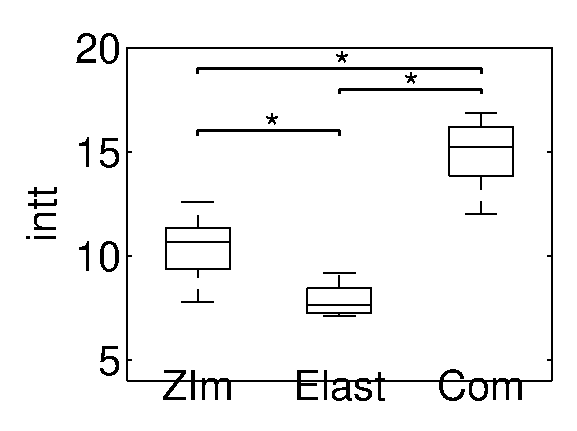
\includegraphics[width=0.3\textwidth]{figures/boxplot.eps}
\caption[Boxplot]{Force $F$ für die Bedingungen $A$, $B$, und $C$.}
\label{fig:boxplot}
\end{figure}
%
\end{comment} 
 



%---------------------------------------------------------------
%DISKUSSION:
%----------------------------------------------------------------

 \section{Diskussion}
 
 Interpretiere deine Ergebnisse. Ist die Leistung akzeptabel? Gehe auf die Ausgangsfragen zurück und vergleiche mit anderen in der Literatur beschriebenen Methoden. Wie erklärst du unerwartete Ergebnisse? Welche Unzulänglichkeiten oder Einschränkungen weisen deine Methoden und Ergebnisse auf? Wo gibt es Raum für Verbesserungen? Könnte eine Kombination mit Methoden aus der Literatur die Arbeit weiter verbessern? Nenne Pläne, Bedürfnisse und Empfehlungen für die zukünftige Forschung. Dies kann auch in einem separaten Unterabschnitt ``Zukünftige Arbeiten'' erfolgen.

%----------------------------------------------------------------
%ZUSAMMENFASSUNG:
%----------------------------------------------------------------

\section{Fazit}
Dies ist keine Zusammenfassung. Hier steht, was das Paper bringt.


%----------------------------------------------------------------%ggf. DANKSAGUNGEN:
%----------------------------------------------------------------

\section*{Danksagungen}
Danken Sie allen, die mit kleineren Ratschlägen oder auf nicht-wissenschaftliche Weise (z. B. technische Unterstützung) beigetragen haben.
%----------------------------------------------------------------

%----------------------------------------------------------------%LITERATUR
%----------------------------------------------------------------

%Latex generates the list automatically from your citations
\bibliography{SampleBibliography}


\end{document}
